\section{Modelo}\label{sec:modelo}

\subsection{Líneas base}
Antes de entrenar la red neuronal se evaluaron tres líneas base con el conjunto de validación. Sin punto de comparación, ninguna métrica de la red significa nada.

\begin{itemize}
  \item \textbf{Baseline 0: \texttt{DummyClassifier}} (\texttt{strategy="most\_frequent"}). El modelo tonto que siempre predice la clase mayoritaria. Demuestra por qué la \emph{accuracy} engaña: alcanza \emph{accuracy} de 0.90 aunque el \emph{recall}-multifatal sea 0.
  \item \textbf{Baseline 1: Regresión logística} (\texttt{class\_weight="balanced"}, \texttt{max\_iter=1000}, \texttt{solver="liblinear"}).
  \item \textbf{Baseline 2: \emph{Random Forest}} (\texttt{n\_estimators=300}, \texttt{class\_weight="balanced"}, \texttt{random\_state=SEED}).
\end{itemize}

\subsection{Arquitectura según N}
Como $3\,000 \leq N < 10\,000$, se aplicó la contingencia C2: Arquitectura A. Tras la búsqueda de hiperparámetros, la corrida ganadora (R5) resultó en una sola capa oculta de 32 neuronas, por lo que la arquitectura final es:

\begin{lstlisting}
model = keras.Sequential([
    layers.Input(shape=(n_features,)),   # 116 caracteristicas
    layers.Dense(32, activation="relu"),
    layers.BatchNormalization(),
    layers.Dropout(0.4),
    layers.Dense(1, activation="sigmoid"),
])
\end{lstlisting}

\subsection{Compilación y pesos de clase}
\begin{lstlisting}
model.compile(optimizer=keras.optimizers.Adam(1e-3),
              loss="binary_crossentropy",
              metrics=[keras.metrics.AUC(curve="PR", name="pr_auc"),
                       keras.metrics.Recall(name="recall"),
                       keras.metrics.Precision(name="precision")])

from sklearn.utils.class_weight import compute_class_weight
w = compute_class_weight("balanced", classes=np.array([0,1]), y=y_train)
class_weight = {0: w[0], 1: w[1]}
\end{lstlisting}
La pérdida utilizada es la entropía cruzada binaria (ecuación de \autoref{sec:marco-teorico}). El peso de clase $w_1$ aumenta el peso de los casos multifatales en la pérdida para compensar el desbalance.

\subsection{Entrenamiento}
\begin{lstlisting}
callbacks = [
    keras.callbacks.EarlyStopping(monitor="val_pr_auc", mode="max",
                                  patience=15, restore_best_weights=True),
    keras.callbacks.ModelCheckpoint("models/letalidad_nn.keras",
                                    monitor="val_pr_auc", mode="max",
                                    save_best_only=True),
    keras.callbacks.ReduceLROnPlateau(monitor="val_loss", factor=0.5,
                                      patience=5, min_lr=1e-5),
]
history = model.fit(X_train, y_train, validation_data=(X_val, y_val),
                    epochs=200, batch_size=32, class_weight=class_weight,
                    callbacks=callbacks, verbose=2)
\end{lstlisting}
Se monitorea el PR-AUC en validación porque es la métrica correcta bajo desbalance. \emph{Early stopping} conserva los mejores pesos. El guardado es en formato \texttt{.keras} de Keras 3.

\begin{figure}[H]
  \centering
  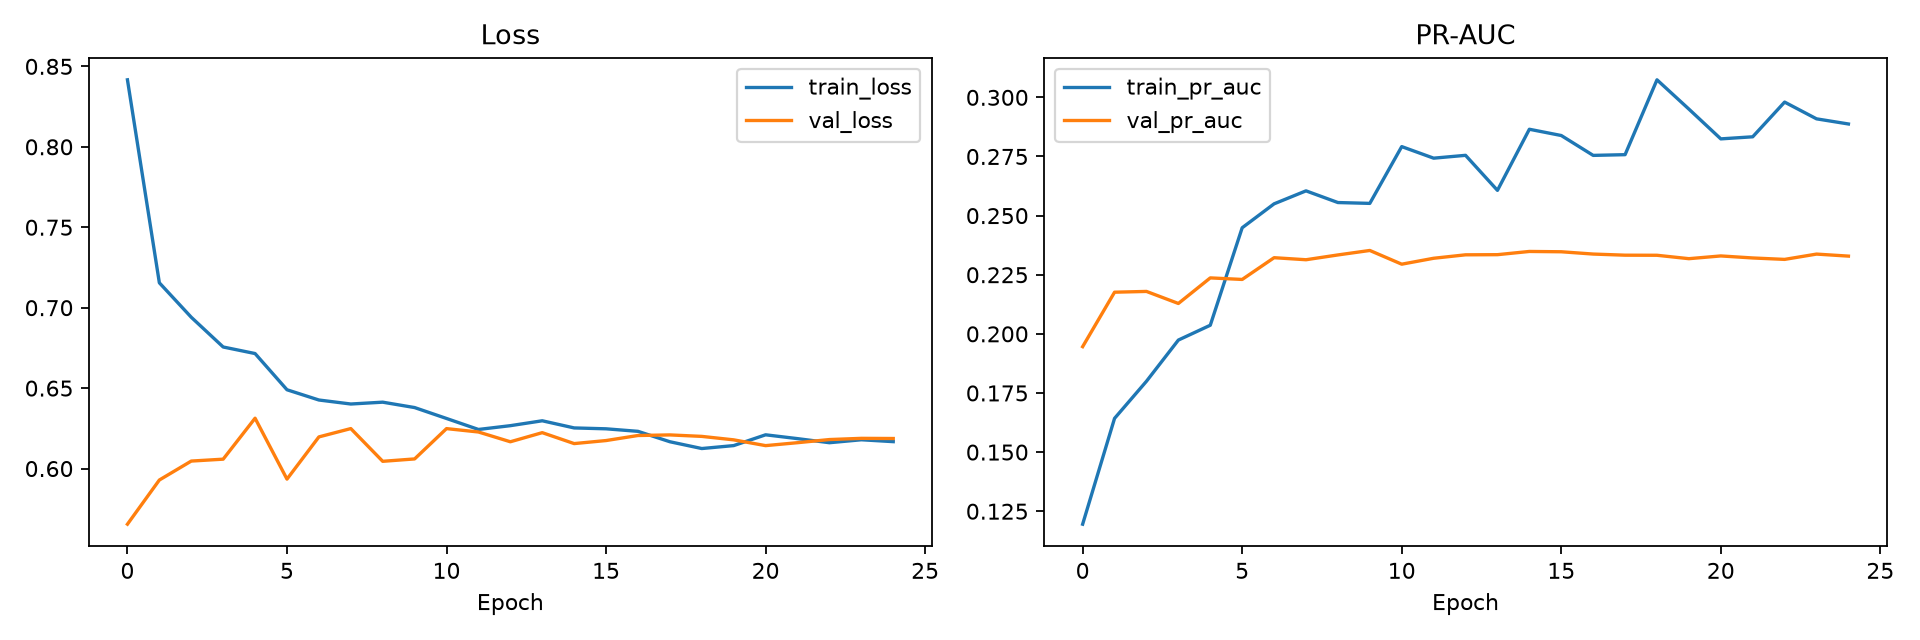
\includegraphics[width=0.8\textwidth]{figures/fig14_training_curves.png}
  \caption{Curvas de pérdida y PR-AUC de entrenamiento vs.\ validación de la corrida ganadora (R5, detenida en la época 22).}
  \label{fig:fig14}
\end{figure}

\subsection{Búsqueda de hiperparámetros: \emph{grid} cerrado de 6 corridas}
El \emph{grid} se definió antes de entrenar: exactamente seis corridas, ni una más ni una menos. La selección fue por mayor F1-multifatal en validación (desempate: PR-AUC). \autoref{tab:grid} resume las seis corridas.

\begin{table}[H]
\centering
\caption{Resultado del \emph{grid} cerrado de 6 corridas en validación (umbral 0.5). Selección por F1-multifatal (desempate: PR-AUC).}
\label{tab:grid}
\begin{tabular}{lccccc}
\toprule
Corrida & Ocultas & Dropout & LR / \emph{batch} & F1-multifatal val & PR-AUC val \\
\midrule
R1 (base)             & 32--16   & 0.4--0.3 & 1e-3 / 32 & 0.2895 & 0.2301 \\
R2 (LR 1e-4)          & 32--16   & 0.4--0.3 & 1e-4 / 32 & 0.2603 & 0.2181 \\
R3 (+0.1 dropout)     & 32--16   & 0.5--0.4 & 1e-3 / 32 & 0.2754 & 0.2365 \\
R4 (mitad neuronas)   & 16--8    & 0.4--0.3 & 1e-3 / 32 & 0.2883 & 0.2312 \\
\textbf{R5 (1 capa)}  & \textbf{32} & \textbf{0.4}   & \textbf{1e-3 / 32} & \textbf{0.2929} & 0.2247 \\
R6 (\emph{batch} 64)  & 32--16   & 0.4--0.3 & 1e-3 / 64 & 0.2481 & 0.2366 \\
\bottomrule
\end{tabular}
\end{table}

\textbf{La mejor corrida fue R5:} una sola capa oculta de 32 neuronas, F1-multifatal en validación de 0.2929. El sobreajuste se controló con \emph{batch normalization}, \emph{dropout} 0.4 y \emph{early stopping} en la época 22.

\subsection{Calibración del umbral de decisión en validación}
Se barrió el umbral de 0.05 a 0.95 en pasos de 0.05 sobre el conjunto de validación. La regla de selección, definida antes de entrenar, privilegia el costo asimétrico: \textbf{máximo \emph{recall}-multifatal entre los umbrales cuyo F1 conserve al menos el 90\,\% del mejor F1 de validación}. \autoref{tab:umbral} (extracto) y la figura~\ref{fig:fig15} muestran el intercambio.

\begin{figure}[H]
  \centering
  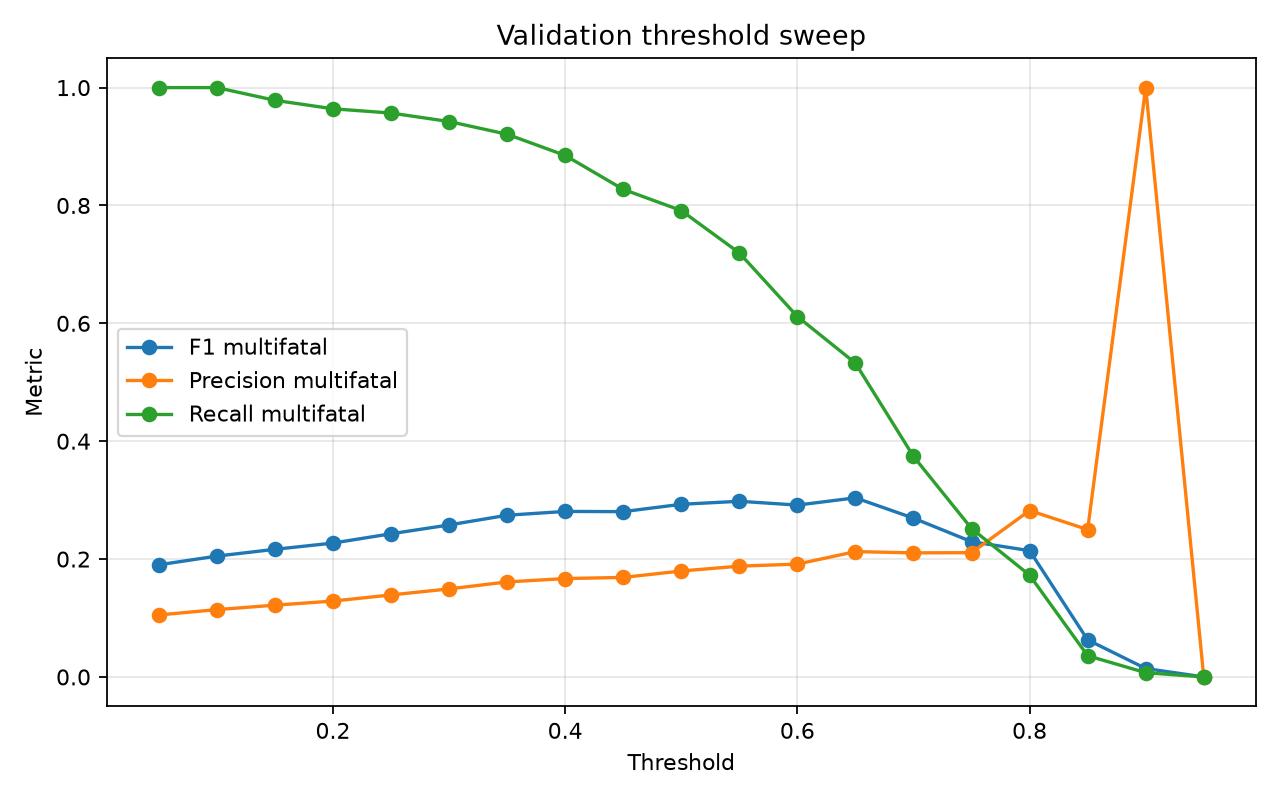
\includegraphics[width=0.8\textwidth]{figures/fig15_threshold_sweep.png}
  \caption{Barrido de umbral en validación. F1, \emph{precision} y \emph{recall} de la clase multifatal vs.\ umbral. El umbral seleccionado (0.35) maximiza el \emph{recall} (0.9209) conservando un F1 dentro del 90\,\% del mejor.}
  \label{fig:fig15}
\end{figure}

\begin{table}[H]
\centering
\caption{Extracto del barrido de umbral en validación (tabla completa en \texttt{tab\_umbral\_validacion.csv}).}
\label{tab:umbral}
\begin{tabular}{cccc}
\toprule
Umbral & F1-multifatal & Precision-multifatal & Recall-multifatal \\
\midrule
0.05 & 0.1903 & 0.1051 & 1.0000 \\
0.20 & 0.2271 & 0.1287 & 0.9640 \\
\textbf{0.35} & \textbf{0.2744} & \textbf{0.1612} & \textbf{0.9209} \\
0.40 & 0.2808 & 0.1669 & 0.8849 \\
0.50 & 0.2929 & 0.1797 & 0.7914 \\
0.65 & 0.3039 & 0.2126 & 0.5324 \\
0.80 & 0.2143 & 0.2824 & 0.1727 \\
0.95 & 0.0000 & 0.0000 & 0.0000 \\
\bottomrule
\end{tabular}
\end{table}

\paragraph{Decisión sobre umbral.} El mejor F1 de validación fue 0.3039 (umbral 0.65), pero con \emph{recall} de solo 0.53: la mitad de los siniestros multifatales pasaría desapercibida. Bajo la regla de costo asimétrico, el umbral 0.35 conserva un F1 de 0.2744 ($\geq$ 90\,\% del mejor) y eleva el \emph{recall} a 0.9209. Se seleccionó 0.35, aceptando explícitamente una precisión baja (0.1612) a cambio de no perder eventos de alta letalidad. Cambiar el umbral después de ver el test habría sido metodológicamente incorrecto; las implicancias operacionales se discuten en la \autoref{sec:discusion}.

\subsection{Persistencia del modelo y artefactos}
Los artefactos canónicos versionados en Git son:
\begin{itemize}
  \item \texttt{models/letalidad\_nn.keras}: el modelo final (corrida R5).
  \item \texttt{models/threshold.json}: el umbral calibrado (0.35) y su regla de selección.
  \item \texttt{models/calibrator.pkl}: el calibrador isotónico post-hoc (ajustado en validación).
  \item \texttt{models/scaler.pkl} y \texttt{models/encoders.pkl}: escalador, codificadores, mapa de frecuencias de vía y categorías cerradas.
  \item \texttt{models/feature\_list.json}: lista ordenada de 116 características (contrato para la GUI).
\end{itemize}
\textbf{El modelo se entrenó una sola vez} (en macOS) y lo consume el otro integrante, sin re-entrenar, para que las cifras del informe sean únicas e indiscutibles. Al cierre del Bloque E, el conjunto de prueba final permaneció \textbf{intacto}: no se evaluó ni una sola vez todavía.